\chapter{Analisi dei Requisiti}

\section{Obiettivi del sistema}


\begin{itemize}
\item progettazione e implementazione dei vari codec in un formato mdc-compatibile
\item progettazione e implementazione di un protocollo per lo scambio dei
flussi di dati in modo \emph{peer-to-peer} (chiamato MDSP)
\item piattaforma per il test dell'insieme
\end{itemize}


\section{Codifica}


Un codec è un dispositivo (hardware o software) in grado di codificare e
decodificare alcune informazioni in un formato di rappresentazione particolare.
In genere il termine è usato in relazione a flussi multimediali (audio/video)
processati tramite un elaboratore elettronico.



\subsection{Modello \emph{Layered}}

TODO: inserire immagine sul modello layered

\subsection{Modello \emph{Multiple Descriptions}}

Il Multiple Description Coding prevede che:
\begin{enumerate}
\item il flusso informativo sia suddiviso in più frammenti, detti 'Descrittori', con circa la stessa quantità di informazioni
\item i descrittori costituiscano due o più sotto-flussi;
\item i descrittori di un solo sotto-flusso, qualunque sia, devono bastare a ricostruire l'informazione, per lo meno con una bassa qualità
\item se vengono ricevuti due o più sotto-flussi, la qualità dell'informazione decodificata aumenta 
\end{enumerate}

TODO: inserire immagine sul modello mdc

\subsection{Differenze tra MDC e Layered}

La principale differenza tra la tipologia di codifica 'a descrizioni multiple' e
quella 'a strati' sta nella differente organizzazione delle informazioni: i
frammenti ottenuti con una codifica MDC hanno potenzialmente lo stesso contenuto
informativo in termini di quantità, mentre nei codec 'layered' esiste un
frammento 'base', più importante degli altri, e diversi frammenti più piccoli di
'avanzamento'.






\section{Testbed}



\subsection{Organizzazione}


Il testbed è composto da un insieme di classi, suddivise in directory:



\begin{itemize}
\item 'common': classi che facilitano la realizzazione delle proprie applicazioni; comprendono utility per accedere alla rete, per simulare un comportamento multi-tasking, e altro.

\item 'codecs': contiene sia classi astratte, da usare come base per i codec
reali, sia classi di utilità, come il registro dei codec, utilizzato per auto-caricare il codec adatto a seconda del flusso informativo

\item 'messages': l'iniseme dei messagi di base
\end{itemize}




\subsection{Implementazione}


Il testbed è stato sviluppato in C/C++, anche se, seguendo le specifiche, è
possibile implementare una qualunque parte del sistema con qualsiasi linguaggio.



\section{MDSP}


MDSP sta per Multiple Description Stream Protocol, ed è un protocollo per lo
scambio di stream di vario tipo (contenuti multimediali) organizzati secondo una
meta-codifica a descrittori multipli.

\begin{figure}[b]
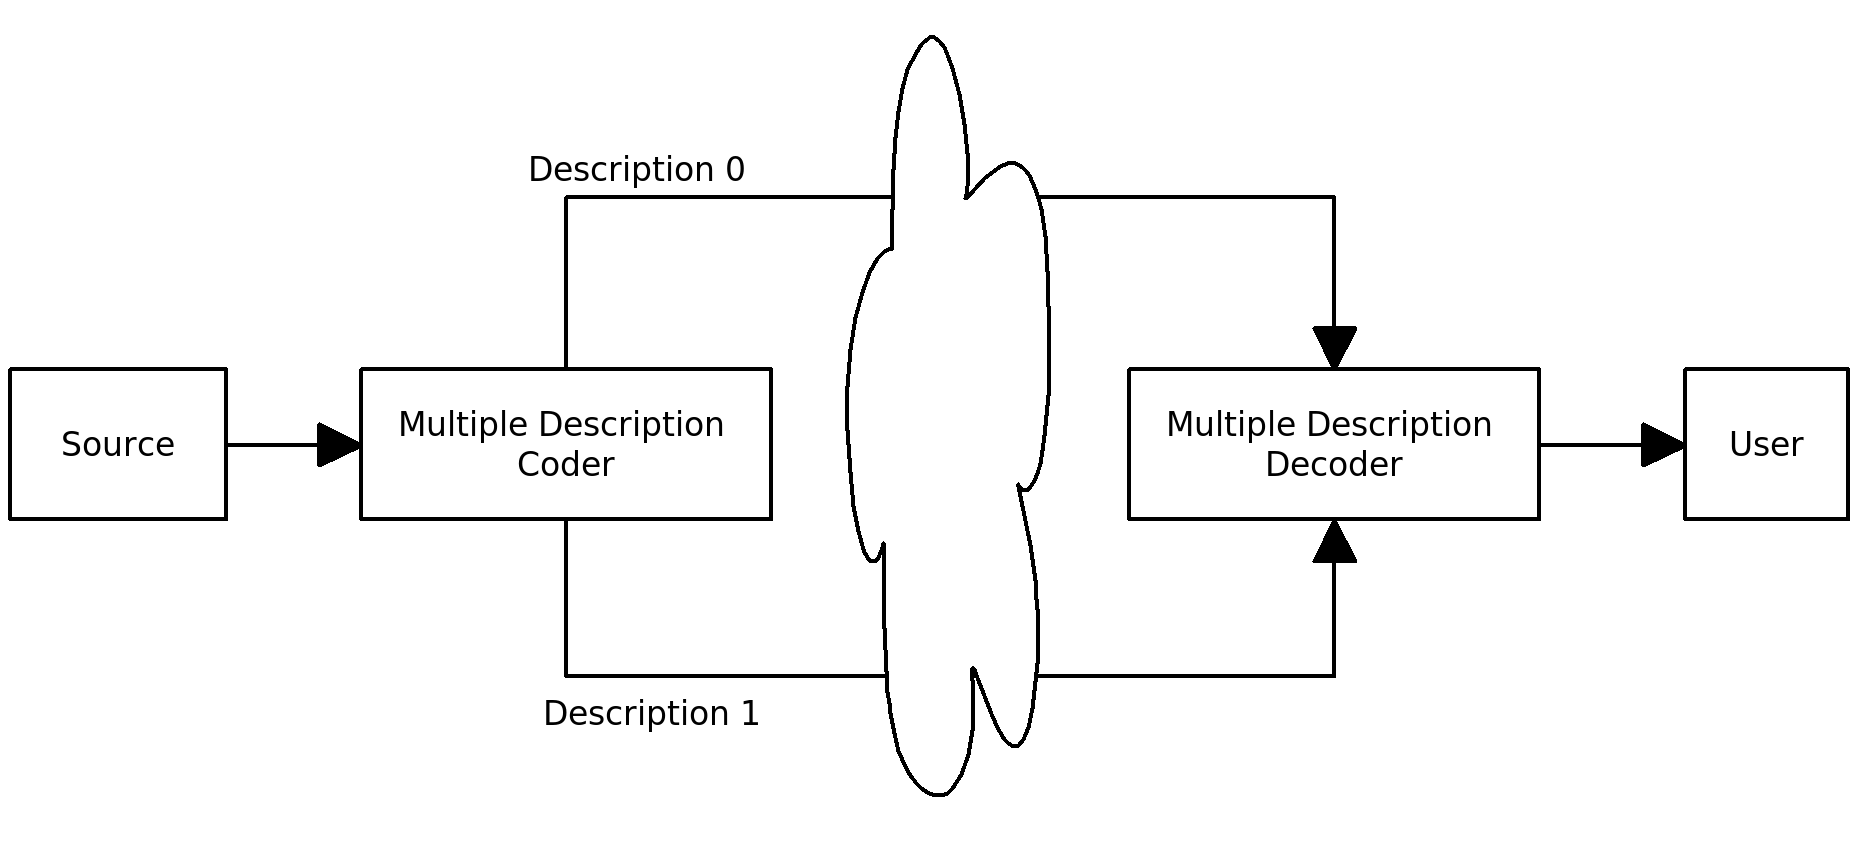
\includegraphics[width=15cm]{../images/network_mdc.png}Richiesta flusso
multimedialeRichiesta liRi
\label{fig:network_mdc}
\caption{Modello di rete basata su MDC}
\end{figure}

\subsection{Casi d'uso}


Chiameremo Alice un generico nodo della rete che vuole effettuare le azioni, e
Bob il peer a cui queste comunicazioni sono dirette.

Ci sono poi anche altri amici, come Carlina, David ed Emy, che condividono le
stesse passioni di Alice e Bob.


\subsubsection{Richiesta di un flusso multimediale}
%

Alice ha bisogno di un flusso multimediale, e sa già che Bob ce l'ha, tutto o in
parte (lo sa perché ha già visto la lista dei flussi di Bob).

Quindi Alice invia un messaggio SREQ, specificando come parametro l'hash univoco
del flusso, il numero della descrizione, e una sequenza di descrittori.

Bob quindi invierà un messaggio ASRQ, specificando come parametro il timeout di
keep-alive; Bob, infatti, continuerà ad inviare il flusso di dati finché riceverà
pacchetti di KALV (keep-alive) da Alice, supponendola disconnessa allo scadere
del timeout.






\subsubsection{Richiesta della lista dei flussi}
%

\begin{itemize}
\item Alice ha bisogno della lista dei flussi disponibili da Bob. Invia un messaggio LIST, non parametro vuoto, e riceve da Bob un messaggio ALST (Answer LiST) contenente un vettore con tutti i nomi e gli hash dei flussi che egli possiede;
\item Alice sta cercando un particolare flusso, di cui sa parte del nome
('pippo'); invia un messaggio LIST a Bob con parametro '*pippo*', e Bob
risponderà con un ALST contenente informazioni su tutti i file che contengono la
parola 'pippo' nel nome.
\end{itemize}




\subsubsection{Richiesta di informazioni su un flusso}
%

Alice sa che un determinato flusso (di cui possiede l'hash) è posseduto da Bob;
invia quindi un messaggio SINF (Stream INFormation), per avere informazioni
specifiche del flusso, ad esempio la durata, la qualità di codifica, ecc. Bob
invia un messaggio ASNF contenente la risposta.






\subsubsection{Invio di parametri di rete}
%

Alice deve informare Bob di cambiamenti che stanno avvenendo dalla sua parte; per
esempio, sta cambiando rete e non vuole interrompere lo streaming; oppure c'è
stato un problema con il router ed è necessario abbassare la velocità di invio
del flusso. In tutti questi casi, Alice invia un messaggio PARM a Bob,
specificando i nuovi parametri.






\subsubsection{Richiesta di altri peer con lo stesso flusso}
%

Alice sta scaricando un flusso da Bob, ma avverte la necessità di frequentare
altre persone, che magari condividono lo stesso flusso; invia quindi un messaggio
PEER a Bob, seguito dall'hash univoco del flusso. Bob raccoglie le idee su tutti
gli amici che conosce, o che ha conosciuto tramite lo scaricamento del flusso in
oggetto, per esempio Carlina, da cui Bob ha scaricato originariamente il flusso,
David, che ha scaricato il flusso tempo fa, ed Emy che lo sta scaricando ora. Bob
quindi prepara un messaggio APER contenente l'indirizzo ip e la porta di Carlina,
David ed Emy e lo invia ad Alice.









